\documentclass[10pt]{article}
\usepackage[landscape,margin=0.55in]{geometry}
\usepackage[T1]{fontenc}
\usepackage{graphicx,amsmath,amssymb,booktabs,longtable,array,xcolor}
\usepackage[colorlinks=true,linkcolor=blue,urlcolor=blue]{hyperref}
\setlength{\parskip}{5pt}
\setlength{\parindent}{0pt}
\setlength{\emergencystretch}{2em}
\newcommand{\Dpp}{D$^{\prime\prime}$}
\begin{document}
\title{Event and waveform supplement: historical}\author{Independent archive reanalysis}\date{13 October 2026}\maketitle
Each event below is a USGS catalog record. Counts refer to traces actually
used in this dataset's images, not all downloaded stations. An asterisk flags a
historical catalog value outside the published magnitude/depth bounds. Both
processed displacement and processed plus source-deconvolved waveforms are shown
for every used trace. Event pages with zero used traces give rejection summaries.
Records retain at least 80 s before S and 65 s after ScS so noise can be assessed.
The blue vertical line marks ScS; red dots mark S. The displacement and deconvolved
curves are each normalized to their own S peak. Display clipping at twice that
amplitude does not alter stored data. SNR is a peak-to-pre-S-RMS ratio.
Receiver splitting corrections have not been applied because the complete original station/path
correction set was not recovered. Phase selection is automatic and requires expert review.
\begingroup\small\setlength{\tabcolsep}{3pt}
\begin{longtable}{llllrrr}
\toprule USGS ID & UTC date/time & Latitude & Longitude & Depth km & Mag/type & Used\\\midrule\endhead
usp0004taw* & 1991-06-23 21:22:28 & -26.802 & -63.349 & 558.0 & 7.3/mw & 0 \\
usp0005te6 & 1993-05-24 23:51:28 & -22.671 & -66.543 & 221.0 & 7.0/mwb & 8 \\
usp000628b & 1993-10-19 04:02:21 & -22.378 & -65.971 & 272.0 & 6.0/mw & 10 \\
usp000669u & 1994-01-10 15:53:50 & -13.339 & -69.446 & 596.0 & 6.9/mwb & 0 \\
usp0006bt7 & 1994-04-29 07:11:29 & -28.299 & -63.252 & 561.5 & 6.9/mwb & 1 \\
usp0006cbq & 1994-05-10 06:36:28 & -28.501 & -63.096 & 600.5 & 6.9/mwb & 0 \\
usp0006h5m & 1994-08-19 10:02:51 & -26.642 & -63.421 & 563.6 & 6.5/mw & 2 \\
usp0007w7v & 1997-01-23 02:15:22 & -21.999 & -65.719 & 276.2 & 7.1/mwc & 10 \\
usp000853a & 1997-07-20 10:14:22 & -22.982 & -66.301 & 256.1 & 6.1/mwc & 0 \\
usp0008bg2 & 1997-11-28 22:53:41 & -13.740 & -68.788 & 586.0 & 6.7/mwc & 23 \\
usp0008u3b* & 1998-08-30 07:52:25 & -23.934 & -66.906 & 219.5 & 5.7/mwc & 4 \\
usp0009eex & 1999-09-15 03:01:24 & -20.934 & -67.275 & 218.0 & 6.4/mwc & 21 \\
usp0009rrz & 2000-04-23 17:01:17 & -28.384 & -62.943 & 609.8 & 6.1/mwc & 1 \\
usp0009suu & 2000-05-12 18:43:18 & -23.548 & -66.452 & 225.0 & 7.2/mwc & 0 \\
usp000ahpv & 2001-06-29 18:35:51 & -19.522 & -66.254 & 273.9 & 6.1/mwc & 0 \\
\bottomrule\end{longtable}\endgroup
The printed historical date 1999-08-30 is inferred to mean 1998-08-30: USGS event usp0008u3b matches the printed latitude and longitude exactly and its depth within 0.5 km. The year correction is an explicit identification assumption; its preferred magnitude of 5.7 is flagged as a historical catalog exception.
\clearpage\noindent\textbf{usp0004taw: 0 used traces; page 1/1}\par
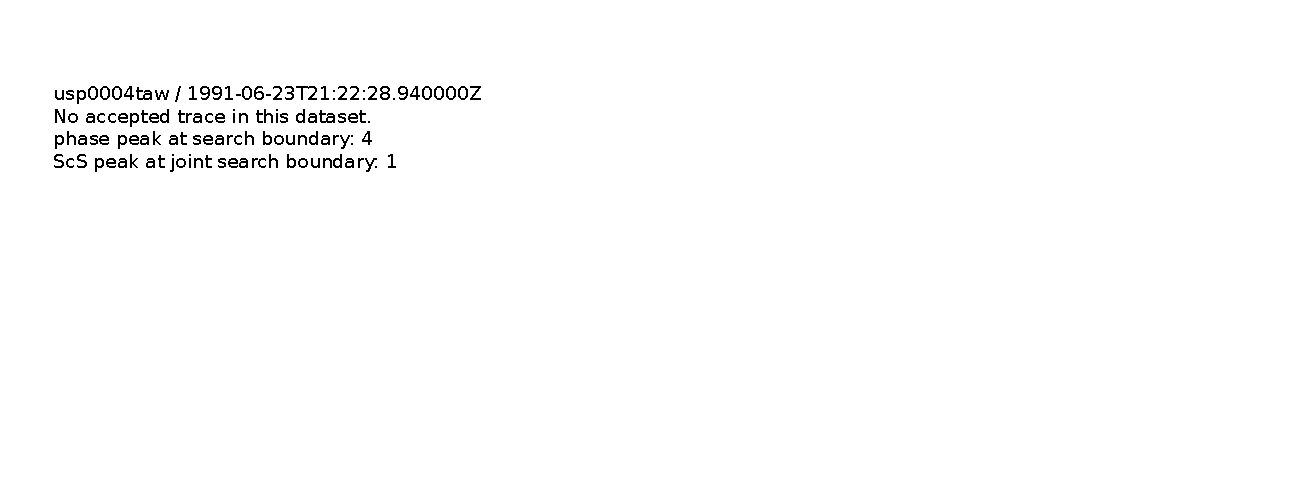
\includegraphics[page=1,width=\linewidth,height=.91\textheight,keepaspectratio]{figures/historical/events/usp0004taw.pdf}
\clearpage\noindent\textbf{usp0005te6: 8 used traces; page 1/1}\par
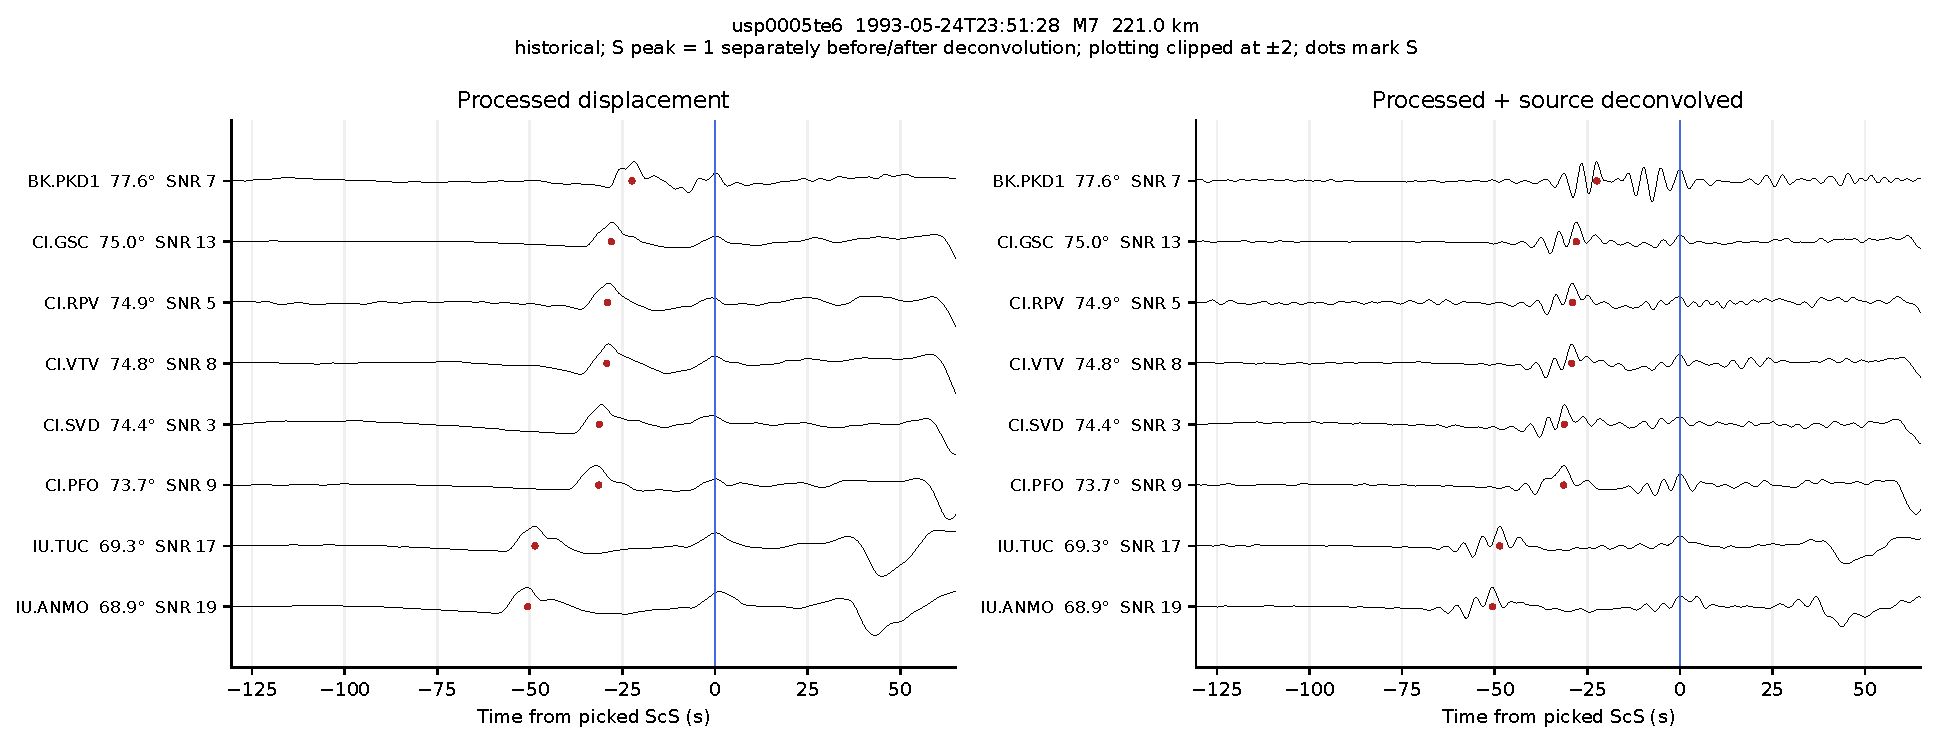
\includegraphics[page=1,width=\linewidth,height=.91\textheight,keepaspectratio]{figures/historical/events/usp0005te6.pdf}
\clearpage\noindent\textbf{usp000628b: 10 used traces; page 1/1}\par
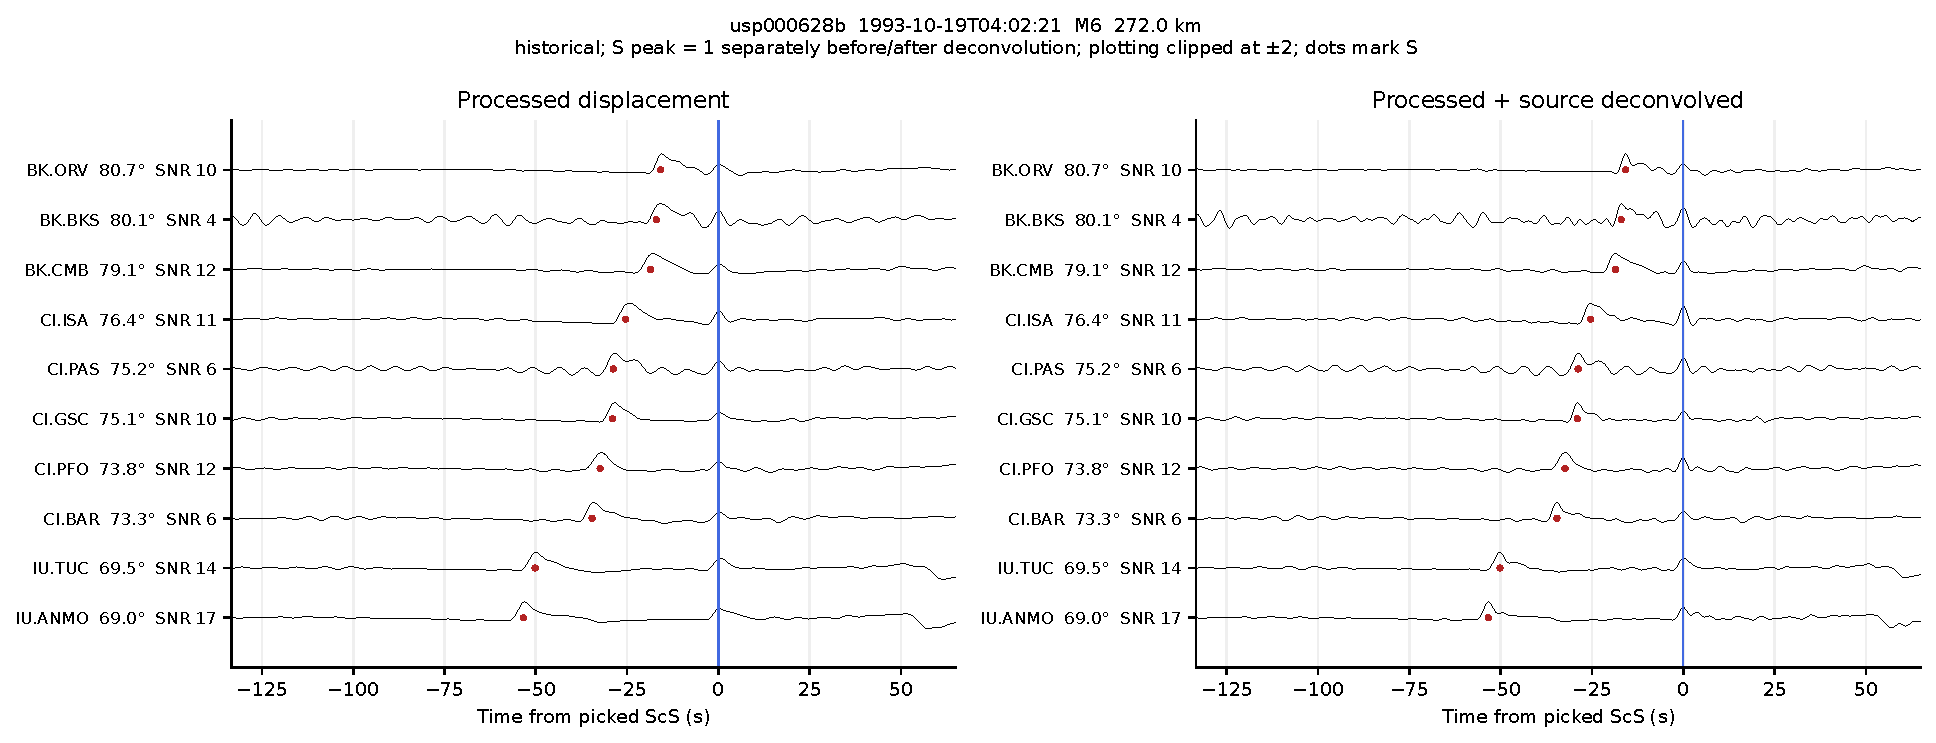
\includegraphics[page=1,width=\linewidth,height=.91\textheight,keepaspectratio]{figures/historical/events/usp000628b.pdf}
\clearpage\noindent\textbf{usp000669u: 0 used traces; page 1/1}\par
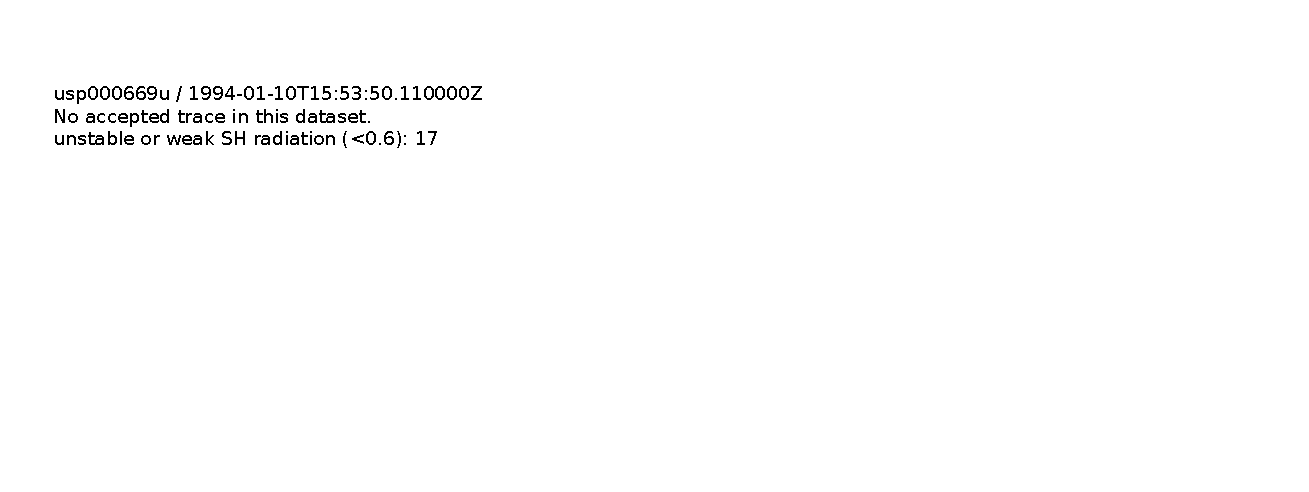
\includegraphics[page=1,width=\linewidth,height=.91\textheight,keepaspectratio]{figures/historical/events/usp000669u.pdf}
\clearpage\noindent\textbf{usp0006bt7: 1 used traces; page 1/1}\par
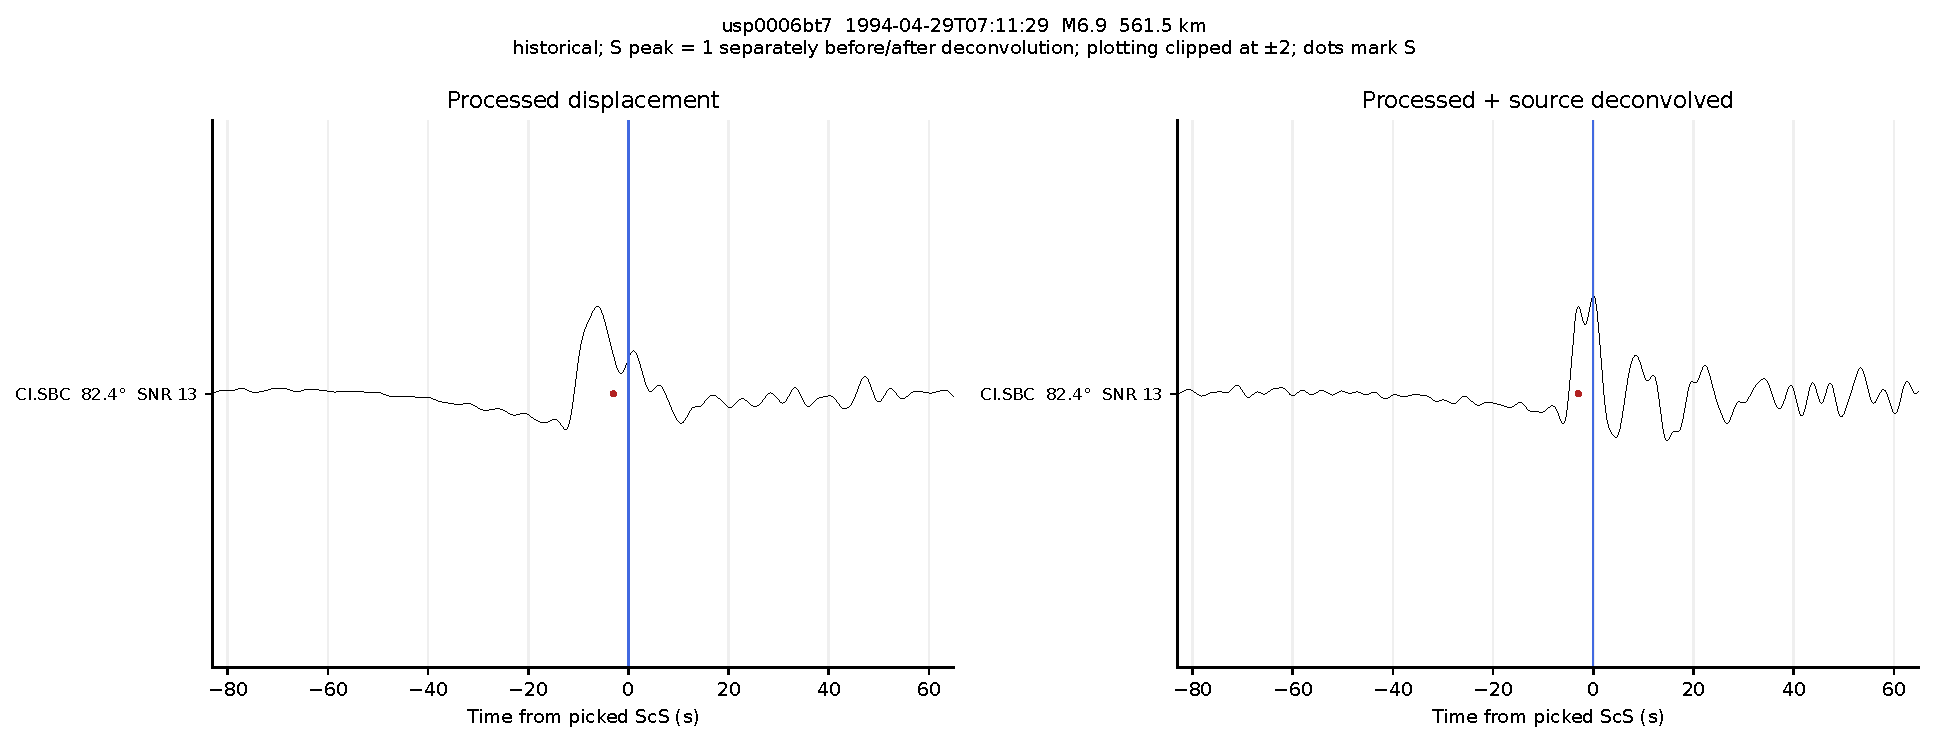
\includegraphics[page=1,width=\linewidth,height=.91\textheight,keepaspectratio]{figures/historical/events/usp0006bt7.pdf}
\clearpage\noindent\textbf{usp0006cbq: 0 used traces; page 1/1}\par
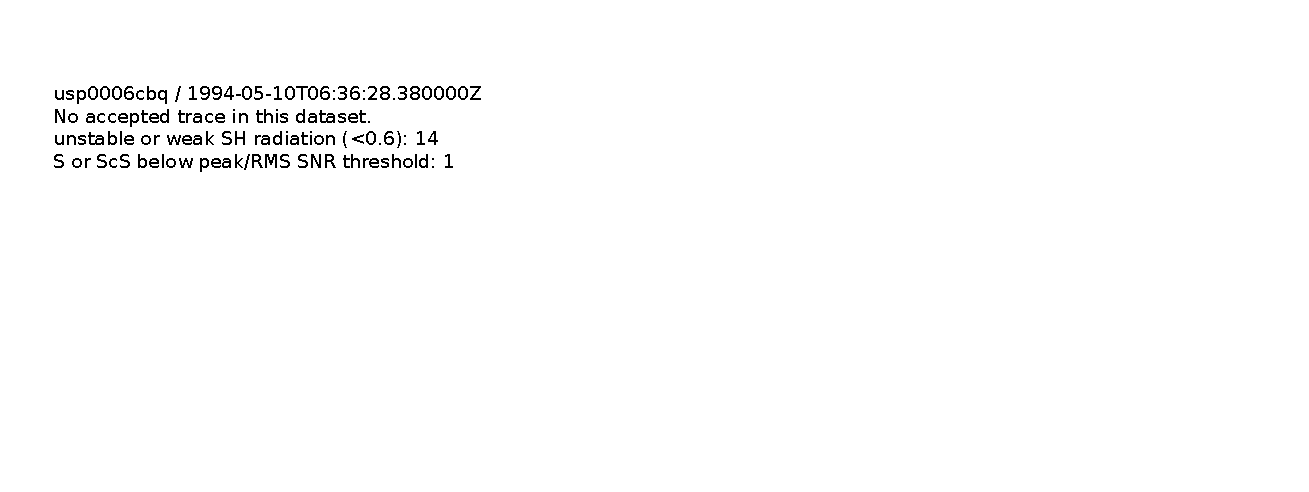
\includegraphics[page=1,width=\linewidth,height=.91\textheight,keepaspectratio]{figures/historical/events/usp0006cbq.pdf}
\clearpage\noindent\textbf{usp0006h5m: 2 used traces; page 1/1}\par
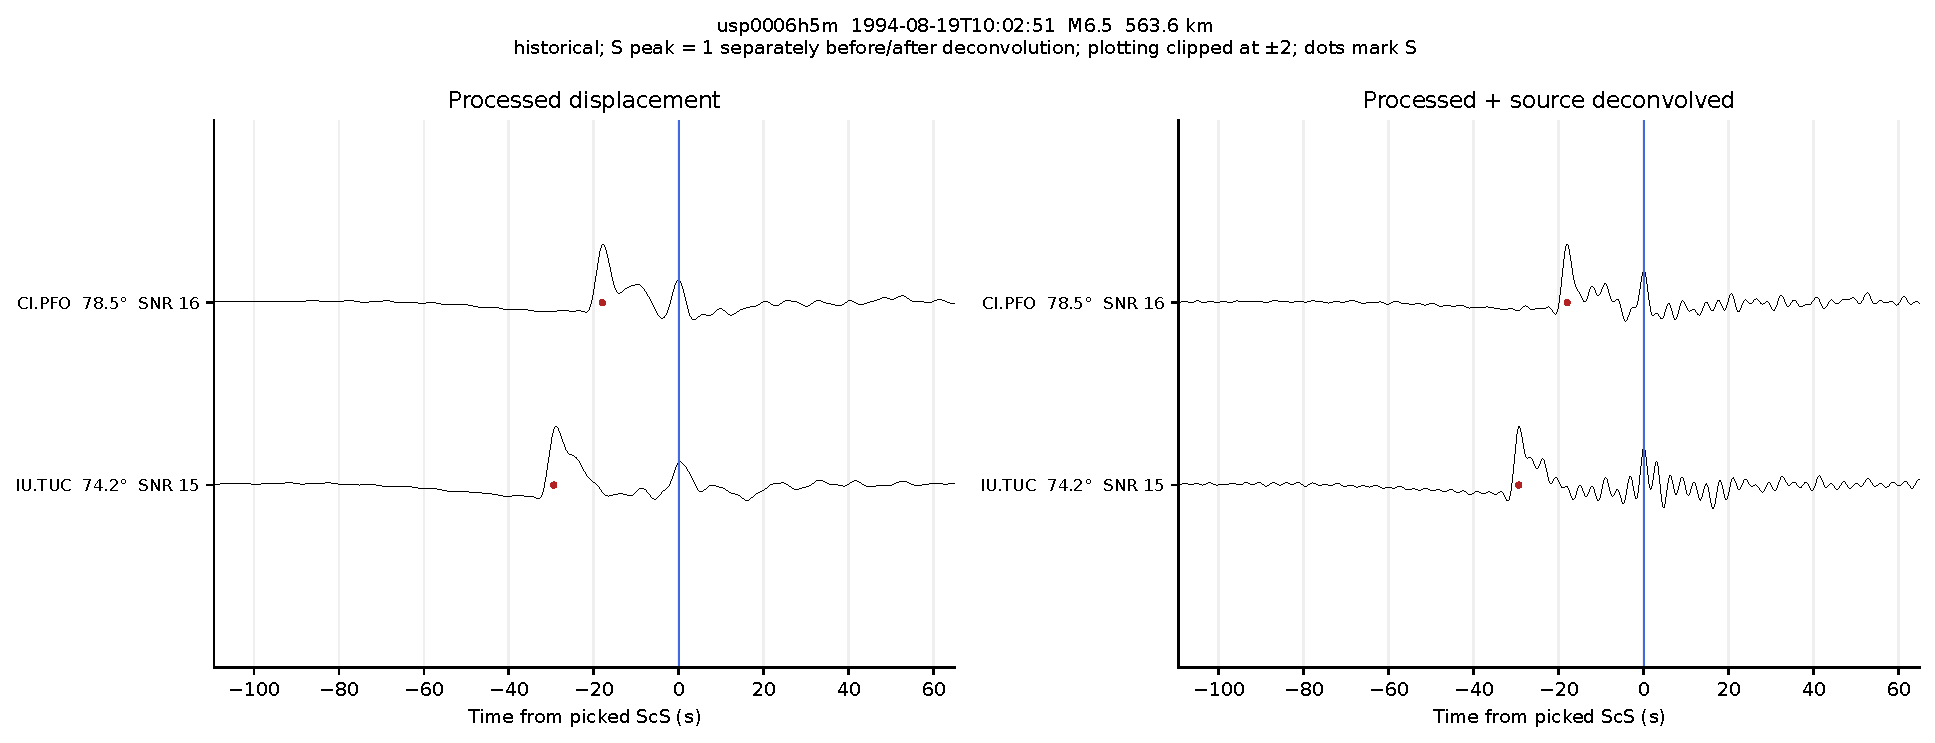
\includegraphics[page=1,width=\linewidth,height=.91\textheight,keepaspectratio]{figures/historical/events/usp0006h5m.pdf}
\clearpage\noindent\textbf{usp0007w7v: 10 used traces; page 1/1}\par
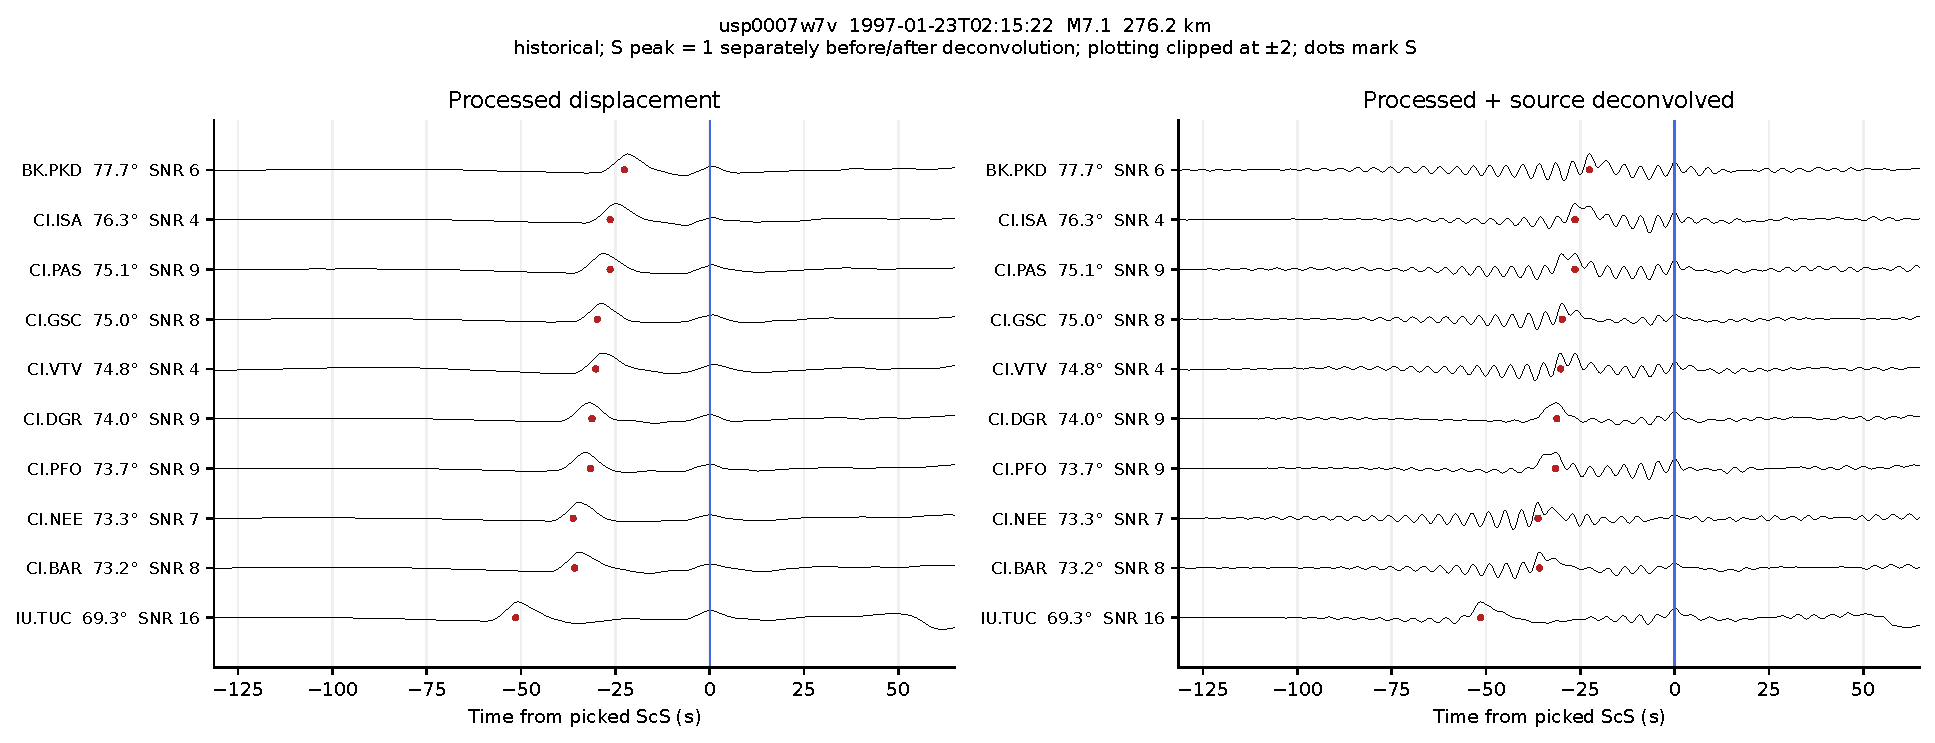
\includegraphics[page=1,width=\linewidth,height=.91\textheight,keepaspectratio]{figures/historical/events/usp0007w7v.pdf}
\clearpage\noindent\textbf{usp000853a: 0 used traces; page 1/1}\par
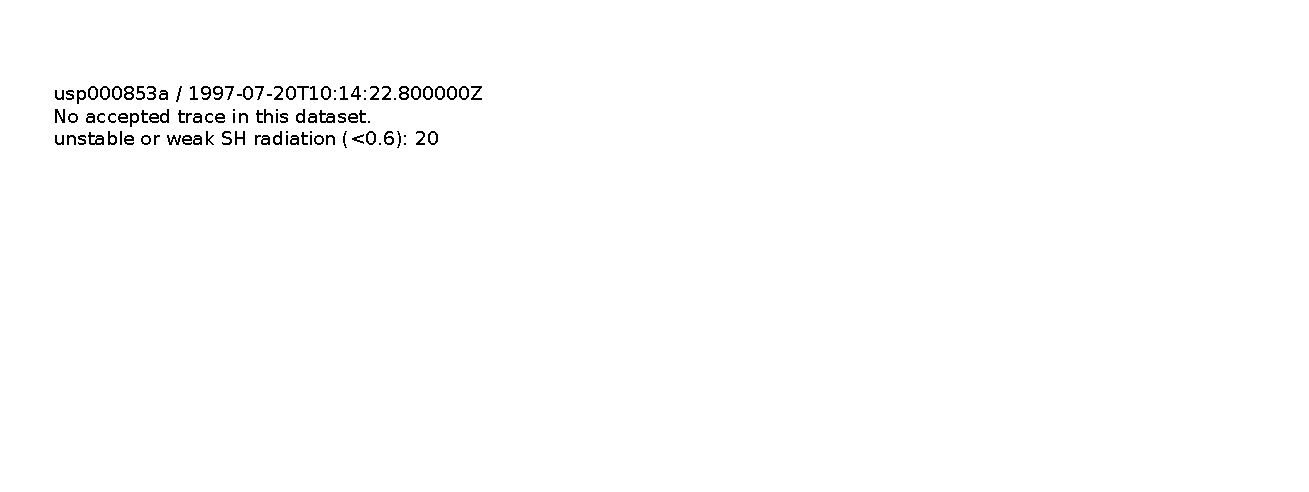
\includegraphics[page=1,width=\linewidth,height=.91\textheight,keepaspectratio]{figures/historical/events/usp000853a.pdf}
\clearpage\noindent\textbf{usp0008bg2: 23 used traces; page 1/1}\par
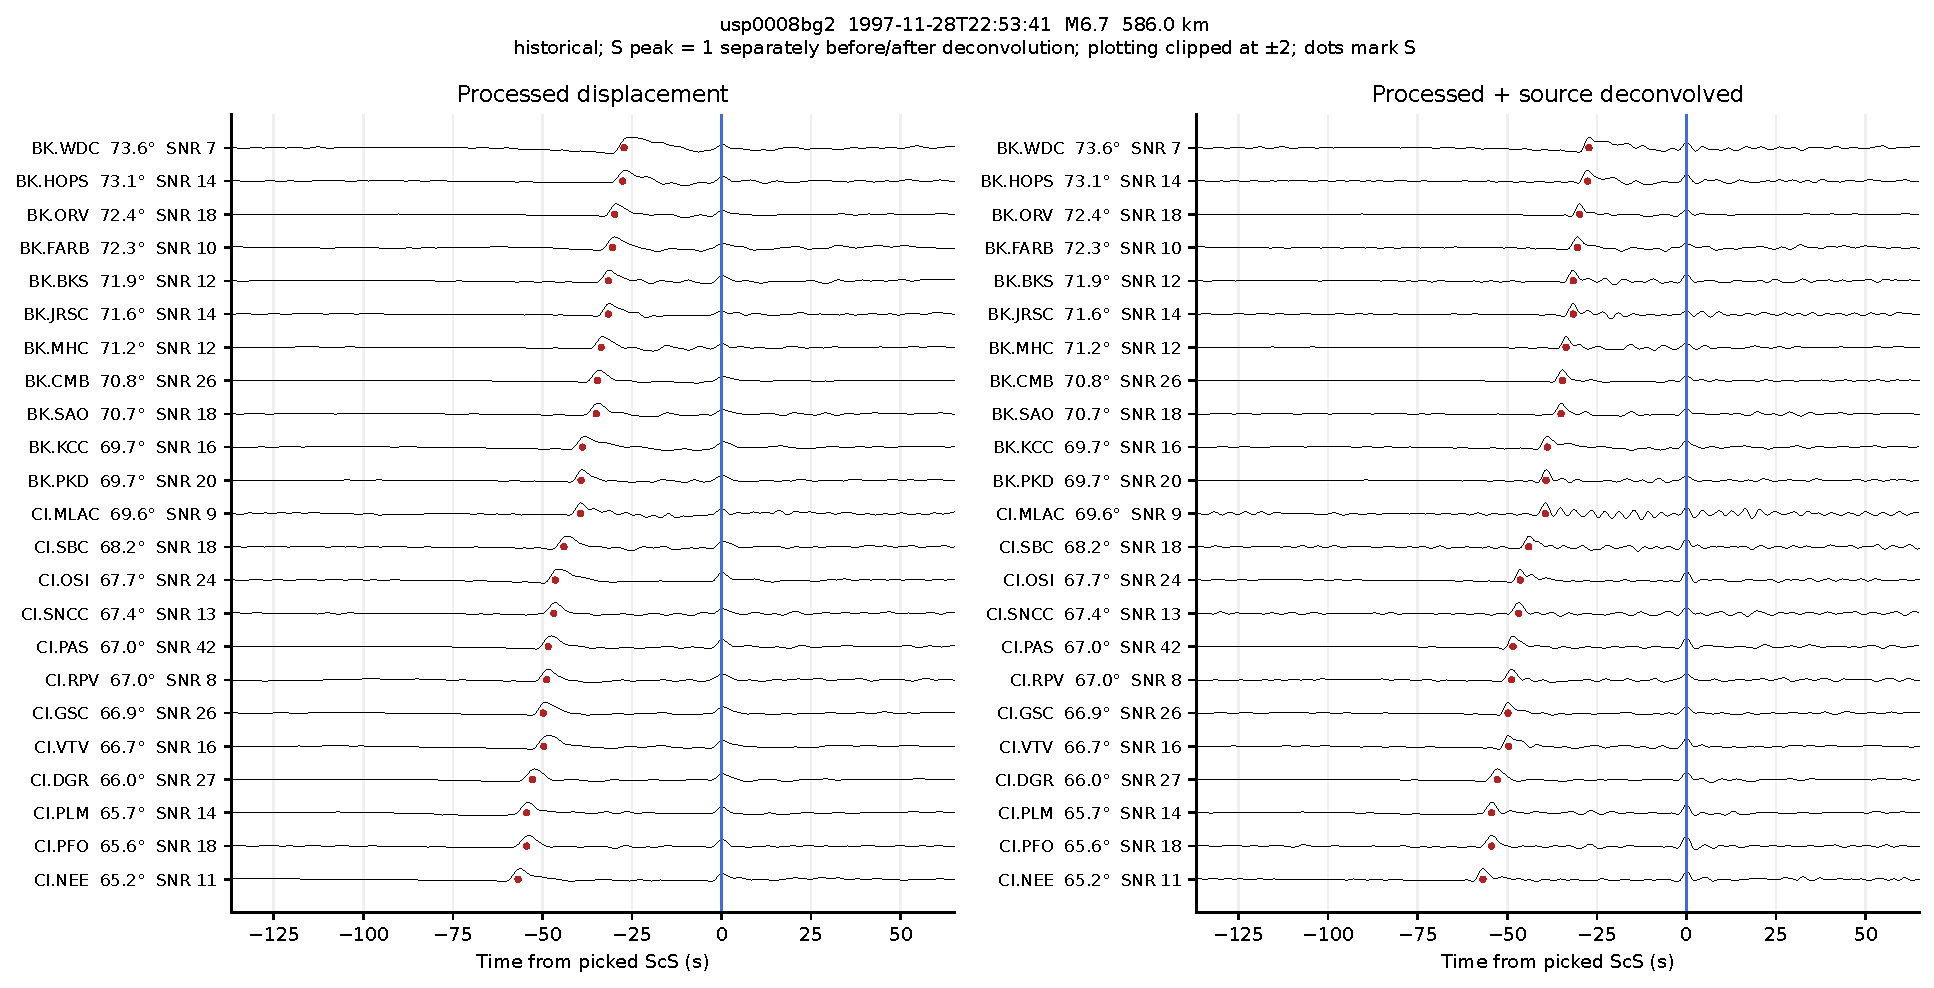
\includegraphics[page=1,width=\linewidth,height=.91\textheight,keepaspectratio]{figures/historical/events/usp0008bg2.pdf}
\clearpage\noindent\textbf{usp0008u3b: 4 used traces; page 1/1}\par
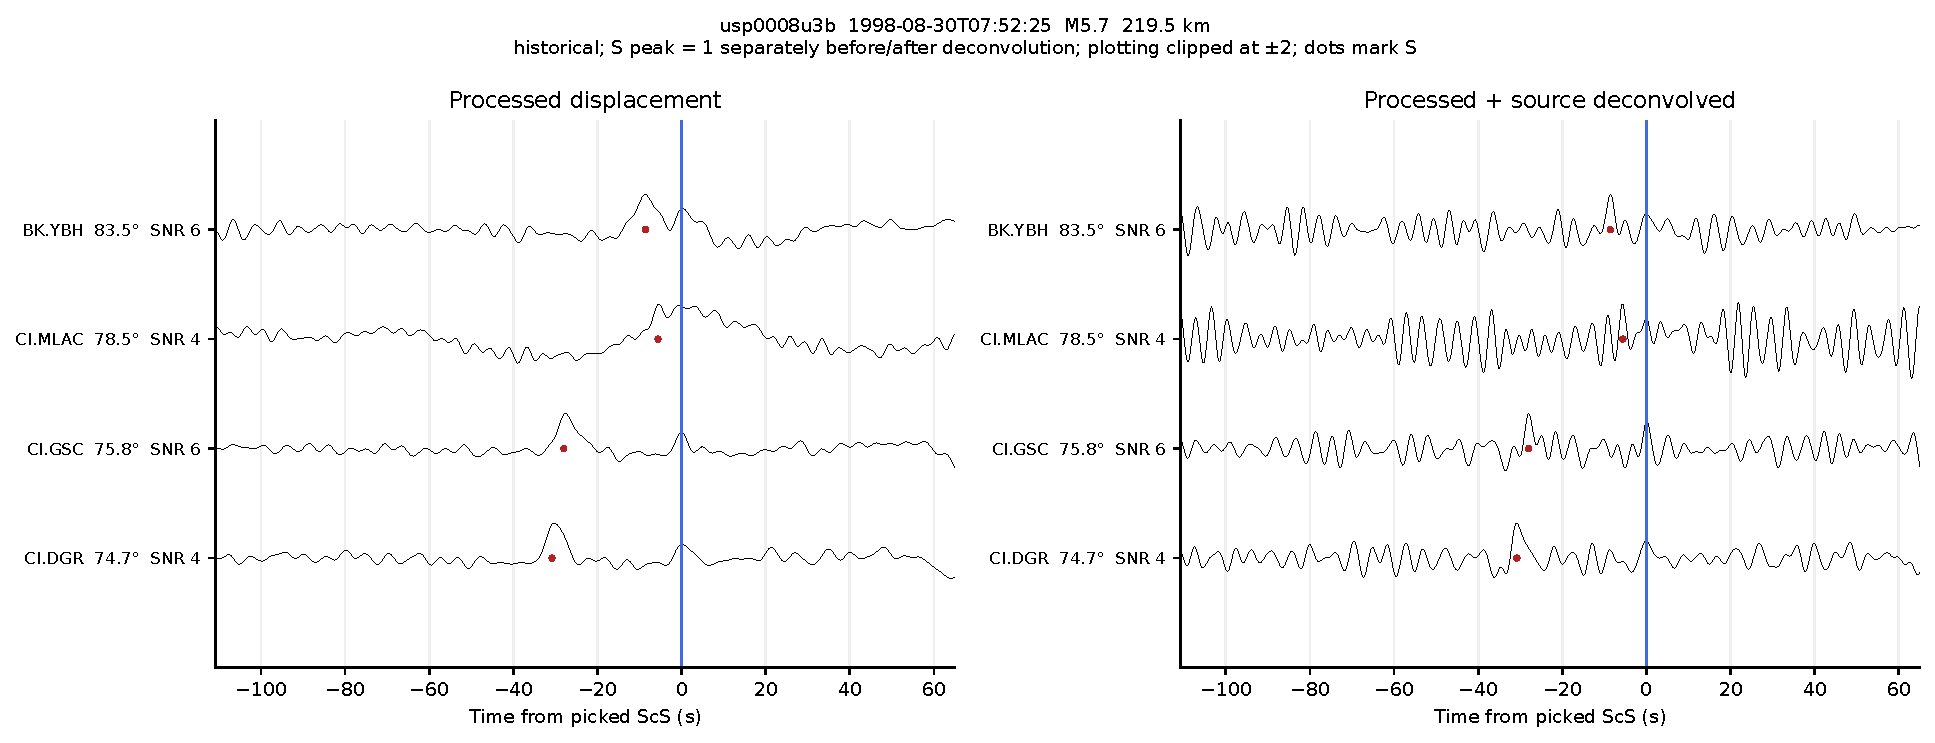
\includegraphics[page=1,width=\linewidth,height=.91\textheight,keepaspectratio]{figures/historical/events/usp0008u3b.pdf}
\clearpage\noindent\textbf{usp0009eex: 21 used traces; page 1/1}\par
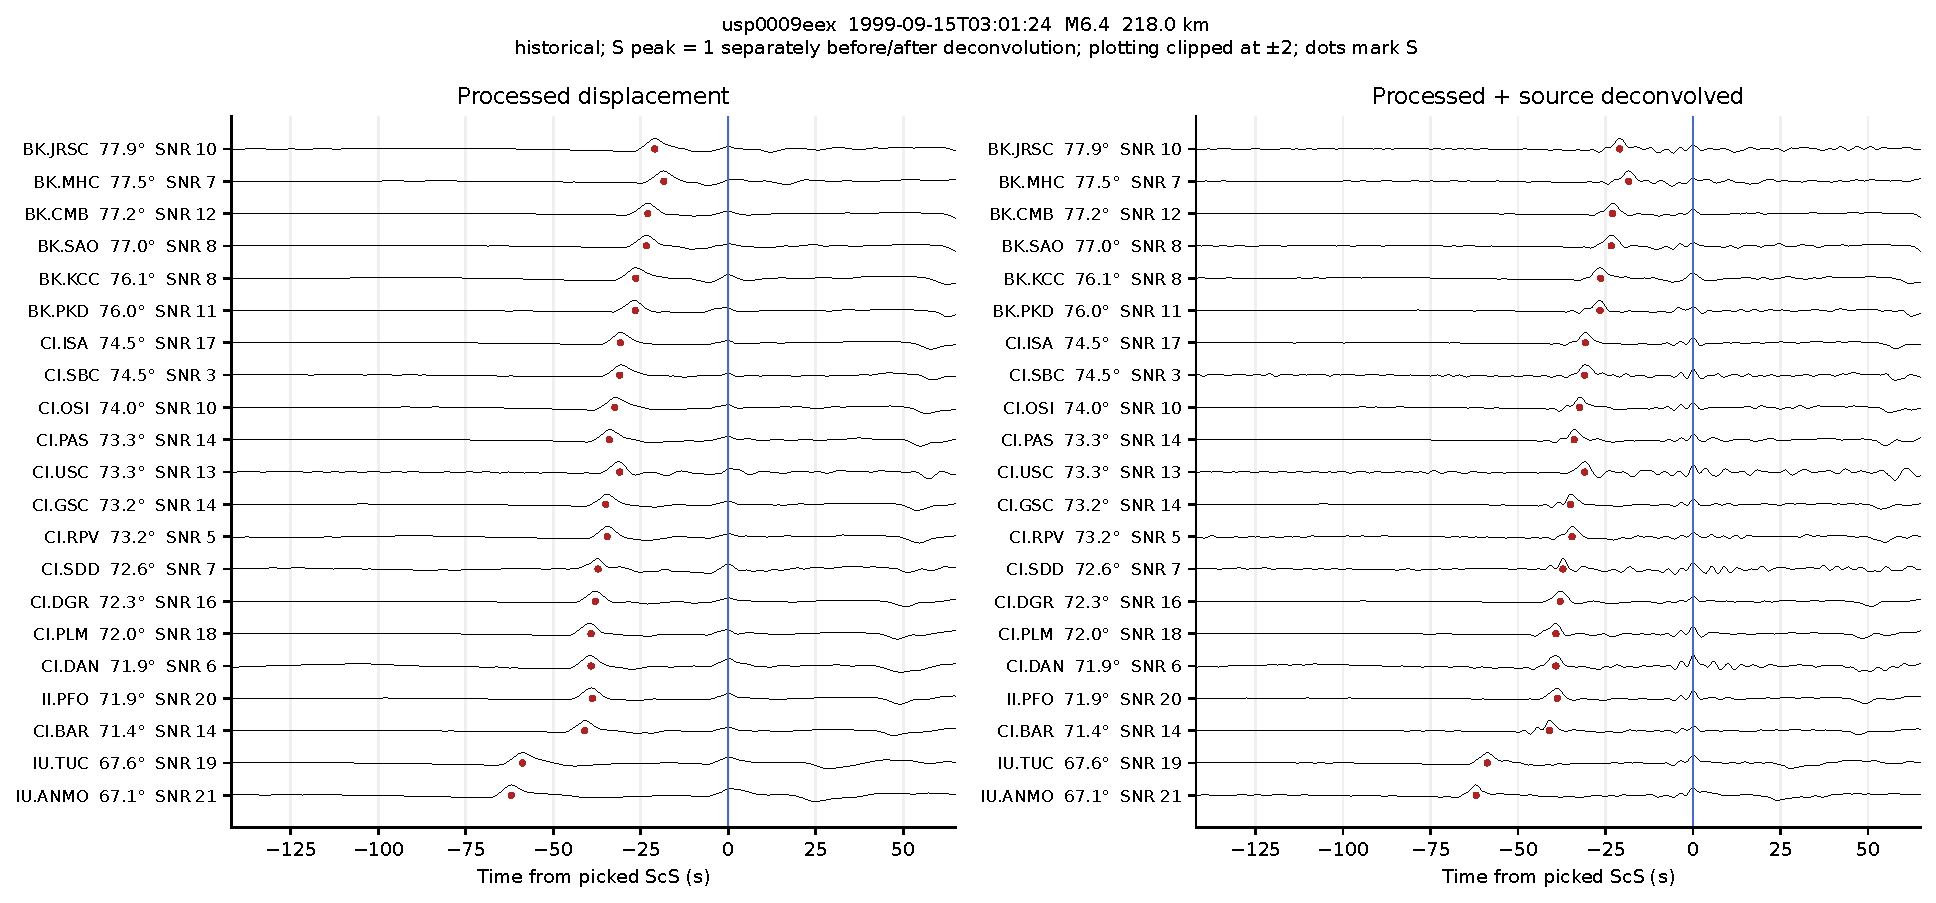
\includegraphics[page=1,width=\linewidth,height=.91\textheight,keepaspectratio]{figures/historical/events/usp0009eex.pdf}
\clearpage\noindent\textbf{usp0009rrz: 1 used traces; page 1/1}\par
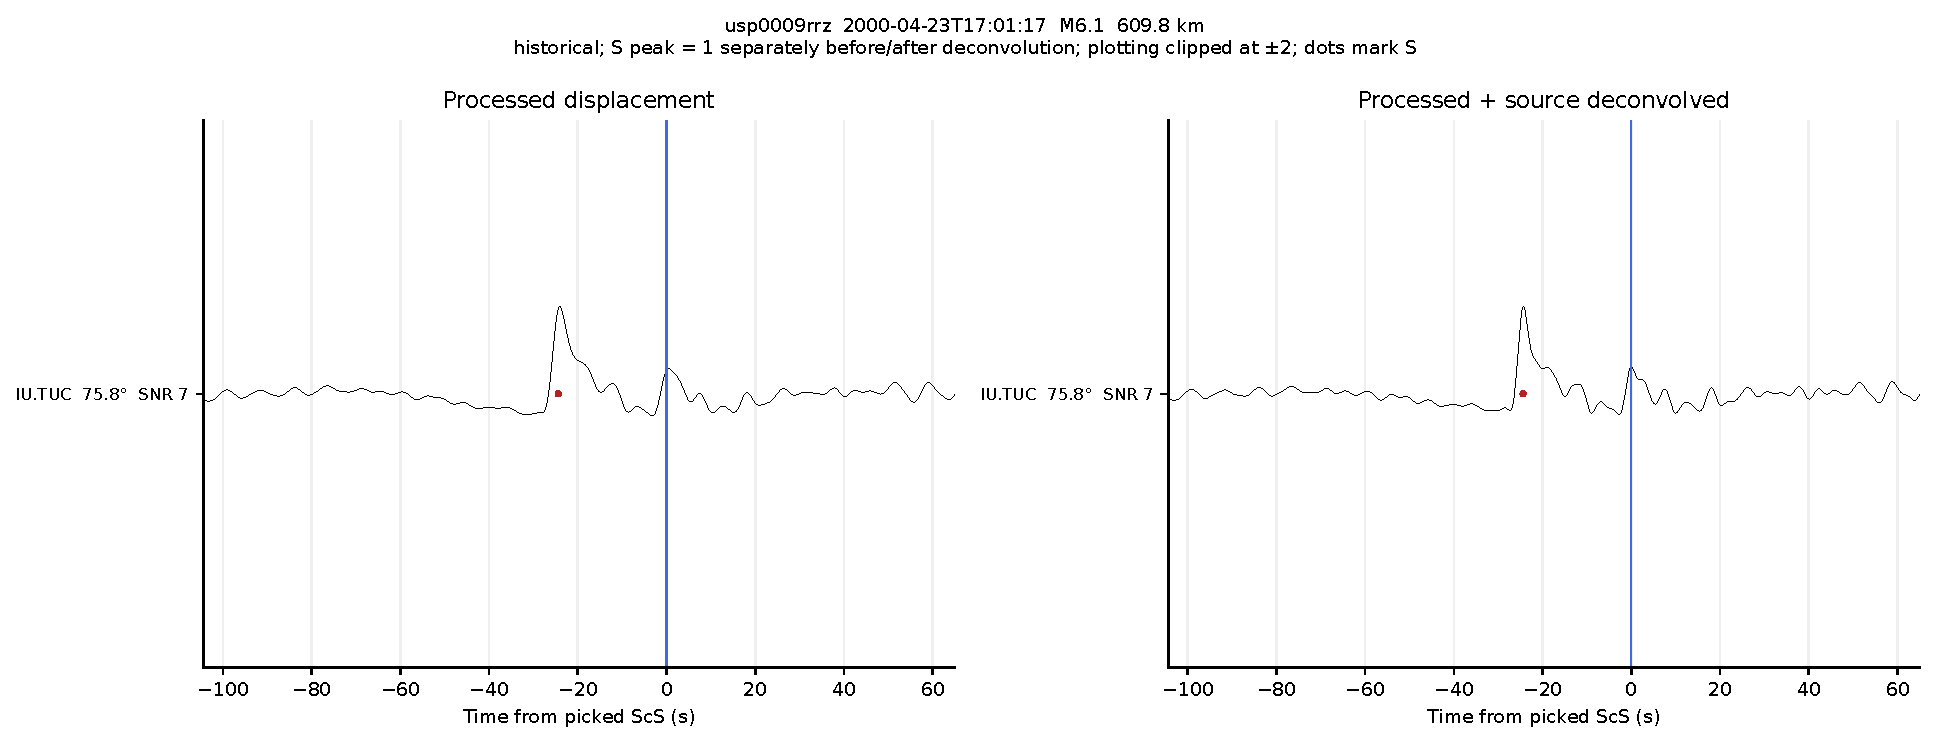
\includegraphics[page=1,width=\linewidth,height=.91\textheight,keepaspectratio]{figures/historical/events/usp0009rrz.pdf}
\clearpage\noindent\textbf{usp0009suu: 0 used traces; page 1/1}\par
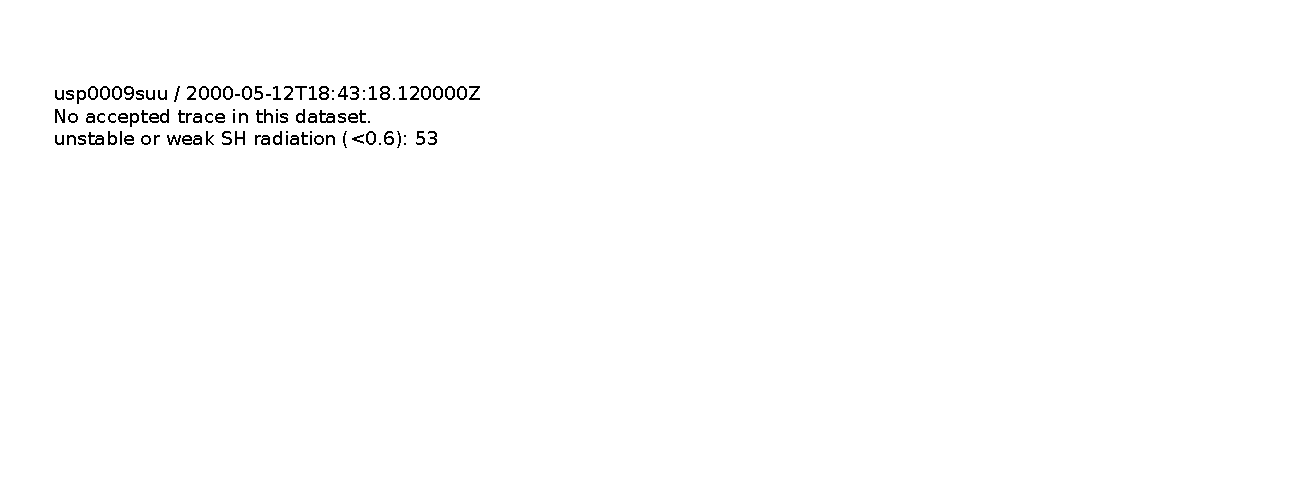
\includegraphics[page=1,width=\linewidth,height=.91\textheight,keepaspectratio]{figures/historical/events/usp0009suu.pdf}
\clearpage\noindent\textbf{usp000ahpv: 0 used traces; page 1/1}\par
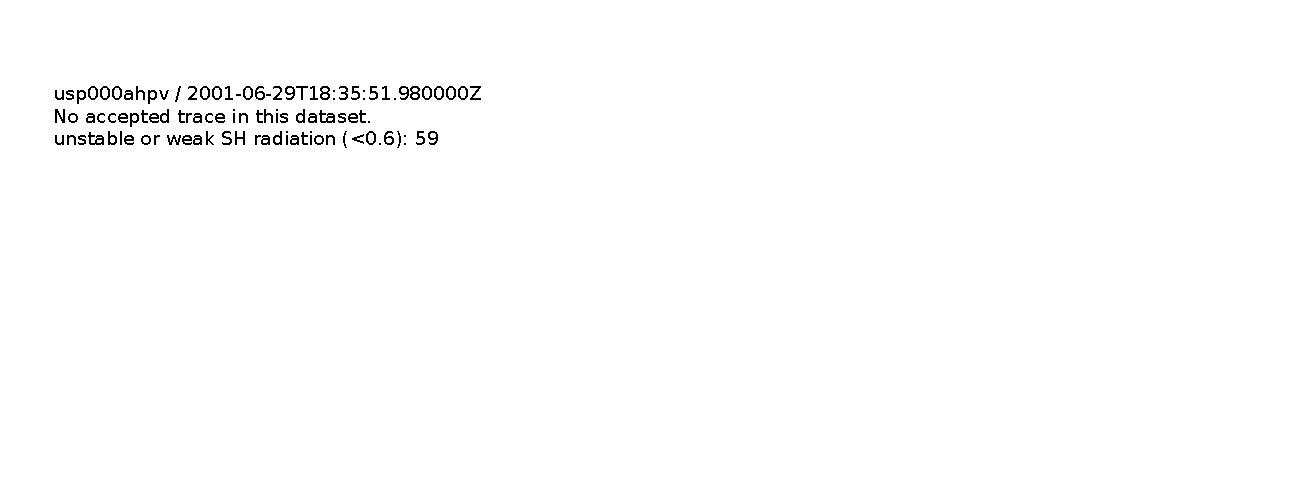
\includegraphics[page=1,width=\linewidth,height=.91\textheight,keepaspectratio]{figures/historical/events/usp000ahpv.pdf}
\end{document}
